\documentclass[11pt]{article}
\oddsidemargin=0.0in
\evensidemargin=0.0in
\textwidth=6.5in
\topmargin=-.25in
\textheight=8.5in
\usepackage{graphicx}
 
\begin{document}
\pagestyle{empty}
 
\begin{center}
{\Large {\bf Linear Algebra Homework Two}}\\
\medskip
{\large {\bf College of the Atlantic}}\\
\medskip
{\large {\bf Due Friday January 18, 2019}}\\
\medskip
\end{center}

\noindent {\bf This assignment is complete.}\\


\noindent Please include a cover sheet for this assignment.\\

\noindent {\bf Chapter 1.3:}
\begin{enumerate}
\setlength{\itemsep}{-1mm}
  \item 5 
  \item 7\footnote{I've reproduced the two slope field figures on the
    last page of this pdf.  You can print this out and draw your
    curves on the figures if you wish.}
  \item In class we considered the logistic differential equation.
    Here we'll examine a modification of that equation:
    \begin{equation}
      \frac{dP}{dt} \, = \, 0.5(P - \frac{P}{100}) - 10 \;.
      \label{eq:logistic}  
    \end{equation}
    Since $P$ describes a population, $P$ is never negative.  We are
    interested only in solutions for $ t \geq 0$.  
    \begin{enumerate}
      \item Sketch the slope field for this differential equation.
        I'd suggest using the desmos tool that is on the Resources
        page on the course web site.  You might have to fiddle around
        with the axes and zoom-level in Desmos for a bit to get a
        useful plot.
      \item Use the slope field to describe the long-term behavior of
        the population.  Does the value of the population at $t=0$
        matter?
        \item What is the biological or practical interpretation of the
          number $10$ in Eq.~(\ref{eq:logistic})?
    \end{enumerate}
    
\item Repeat parts (a) and (b) of the above question, but with the
  following, slightly different, differential equation:
  \begin{equation}
    \frac{dP}{dt} \, = \, 0.5(P - \frac{P}{100}) - 20 \;.
    \label{eq:logistic2}  
  \end{equation}
\end{enumerate}

\noindent {\bf Chapter 1.4:}
\begin{enumerate}
\setlength{\itemsep}{-1mm}
  \item 2
  \item 13
  \item 22
  \item 35
  \item 49
  \item 51
    
\end{enumerate}

\noindent {\bf Chapter 1.5:}
\begin{enumerate}
\setlength{\itemsep}{-1mm}
  \item 3
  \item 14
\end{enumerate}


\begin{figure}[h]
\vspace{-8mm}
\begin{center}
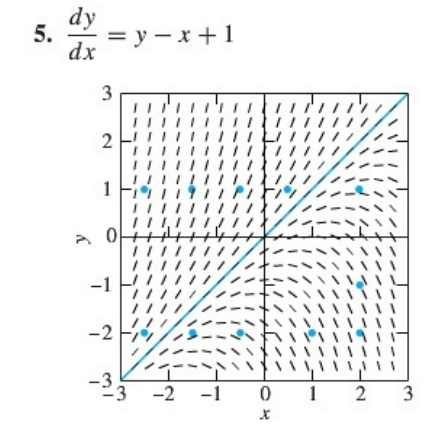
\includegraphics[width=4in]{slopefield_1.png}
\vspace{-2mm}
\caption{The slope field for problem 5 from Chapter 1.3.}
\vspace{-5mm}
\end{center}
\end{figure}

\begin{figure}[h]
\vspace{-2mm}
\begin{center}
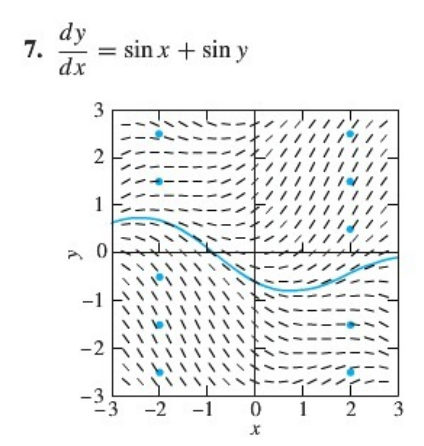
\includegraphics[width=4in]{slopefield_2.png}
\vspace{-2mm}
\caption{The slope field for problem 7 from Chapter 1.3.}
\vspace{-5mm}
\end{center}
\end{figure}


\end{document}
